\subsection{UCP}
\label{sec:algorithms:ucp}

\gls{ucp}~\cite{Qureshi2006} was first presented in 2006. 
\gls{ucp} uses the concept of utility when assigning ways to a core.
Using a \gls{umon}, \gls{ucp} divides the ways in the cache between the cores.
\gls{ucp} then uses the same insertion and promotion policy as \gls{lru}.
The replacement policy is as in \gls{lru} but with two modifications:
First if the number of blocks owned by the requesting core is less than the number of ways assigned to it, then the least recently used block that is not assigned to the requester core is replaced.
If however the number of blocks owned is greater than or equal to the number of assigned ways the replacement algorithm selects the least recently used block of those owned by the requester.
This replacement policy ensures that the division between cores in each set move toward the global allocation following cache misses.
At the same time, a core may use more blocks that it is currently assigned, given that the space is not claimed by any other core.

The \gls{umon} is the core of the \gls{ucp} algorithm.
It consists of one \gls{atd} per core sharing the cache. 
The \gls{atd} is managed by normal \gls{lru} replacement and has one access counter per way.
Whenever a cache request hits in the \gls{atd}, the access counter representing the way the block was in is incremented.
In other words, \gls{umon} uses the stack property of \gls{lru}, as explained in Section~\ref{sec:algorithms:lru}, to find the hit rate of all valid partition sizes.
In addition to the \glspl{atd}, there is a monitor circuit that uses the access counters to calculate a new global partition at set intervals.
In the original paper, the authors recalculate the partitioning every 5M cycles.

The original paper proposes several algorithms for determining optimal partitioning based on the counter data. 
One of them is the Lookahead Algorithm suitable when there are more than two cores sharing a cache.
The Lookahead Algorithm assigns ways based on an increase in marginal utility; it is given in Algorithm~\ref{alg:algorithms:ucp}.
While there are more ways to distribute, the algorithm calculates the maximum marginal utility achievable by each core. 
The core with the highest value wins and is assigned as many ways as needed to achieve the increase.
The algorithm continue until all ways have been assigned.
Lines 27-28 calculate the marginal utility. 
First the number of misses prevented by increasing the allocation from a to b is found.
Due to the stack property of \gls{lru}, this is simply done by summing the access counters for ways $a$ to $b-1$.
The number of misses is then divided by the number of sets introduced, to find the marginal utility.
The rest of the algorithm is simply a greedy algorithm selecting the highest marginal utility at each iteration.
After a reallocation of cache ways, the \gls{atd} counters are all halved.
By doing this, the \gls{umon} will keep historical data for future decisions while prioritizing data from the current period.

Because the lookahead algorithm is greedy, finding a case where it makes a non-optimal choice is rather easy.
Consider a case with two cores, and two ways left to assign.
By assigning one way to core 0 it will receive 10 more hits, 2 ways offers no improvement.
Assigning one way to core 1 causes no additional hits, but if given two ways it will receive 18 hits.
In this case, the marginal utility is 10 for core 0 and 9 for core 1.
The algorithm assigns one way to core 0, and in the next iteration both have zero utility and it does not matter which is assigned the last way.
In this case, the algorithm saved 10 misses while it could have saved 18.
In order to guarantee optimal decisions the algorithm would have to do an exhaustive search of the solution space, but this is infeasible as it requires a lot more resources than the simplified greedy algorithm.

\begin{figure}[t]
    \centering
    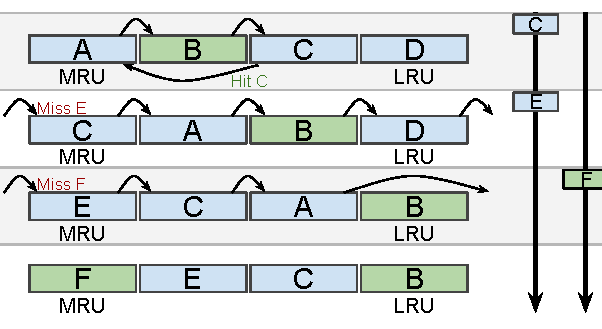
\includegraphics[width=.65\textwidth]{figures/algorithms/UCP}
    \caption[UCP managed 4-way cache set.]{UCP managed 4-way cache set. (Two cores each allocated two blocks)}
    \label{fig:algorithms:ucp_example}
\end{figure}

Figure~\ref{fig:algorithms:ucp_example} show an example cache set managed by \gls{ucp} shared by two cores.
We assume that both cores are allocated two blocks.
Initially, core 0 has three blocks in the cache as indicated by the blue background color; A, C, and D.
The first request is by core 0 for block C; this is a hit causing the block to be promoted to \gls{mru}, pushing A and B towards the \gls{lru} position.
Next is a request for E by core 0; this is a miss.
Because core 0 already has more than the number of allocated blocks in the cache, the block closest to \gls{lru} owned by core 0 is evicted, D in this case.
Finally, a request for F is made by core 1; this is also an miss.
Because core 1 has less than the number of allocated blocks in the cache, a block not owned by core 1 is to be evicted.
As a result, B owned by core 1 at the \gls{lru} position is saved, and rather A at the next to \gls{lru} position is evicted.



\begin{algorithm}[ht]
\caption{UMON Lookahead Algorithm.}
\label{alg:algorithms:ucp}
\begin{algorithmic}[1]
\State $balance\gets N$ /* Number of ways */
\State $allocations[i]\gets 0$ /* for each core $i$ */
\While {$balance$}
    \ForAll {$cores\ i$}
        \State $alloc\gets allocatations[i]$
        \State $max\_mu[i]\gets \Call{get\_max\_mu}{i, alloc, balance}$
        \State $blocks\_req[i]\gets$ min blocks to get max\_mu[i] for i
    \EndFor
    \State $winner\gets$ application with the maximum value of max\_mu
    \State $allocations[winner] += blocks\_req[winner]$
    \State $balance -= blocks\_req[winner]$
\EndWhile
\State \Return alloactions
\State

\Function{get\_max\_mu}{$i, alloc, balance$}
    \State $max\_mu\gets 0$
    \For{$ii = 1; ii <= balance; ii++$}
        \State $mu\gets \Call{get\_mu\_value}{p, alloc, alloc+ii}$
        \If{$mu \ge max\_mu$}
            \State $max\_mu\gets mu$
        \EndIf
    \EndFor
    \State \Return{$max\_mu$}
\EndFunction
\State

\Function{get\_mu\_value}{$p, a, b$}
    \State $U\gets$ change in misses for application p when number of blocks assigned to it increases from a to b
    \State \Return{$\frac{U}{b-a}$}
\EndFunction
\end{algorithmic}
\end{algorithm}